Given two sets $A, B \subseteq \mathbb{N}$ we want to compute:
$$
    A \cap B = \{ x : x \in A, x \in B \}
$$

That problem is useful in database JOINS operations and in search engines too where we have a dictionary for each search term and associated to it we have the list of document IDs who contains that search term, so when we are looking for results of a query we want the documents who contains all the terms, so the intersection between the dictionary associated elements.

Throughout all the algorithms we will see we assume that sets are sorted, because otherwise the only algorithm is the for loop inside a for loop which in case $|A|=n $ and $|B|=m$ it's $O(m \cdot n)$ time which is very bad!

\section{Common approaches}
\subsection{Merge-based intersection}
It's derived from the merge procedure from merge-sort.
Take for example $A = \{ 1, 5, 8, 9, \_ \}$ and $B = \{ 2, 5, 9, \_ \}$, we take two pointers at the start of the lists and we move the one that points to the smallest element at each comparison, when both points to the same element we get a match and save it.
So for example:
\begin{itemize}
    \item we check 1 from $A$ and 2 from $B$, no match, we move $p_A$;
    \item we check 5 from $A$ and 2 from $B$, no match, we move $p_B$;
    \item we check 5 from $A$ and 5 from $B$, we have a match, yield the item and move both $p_A$ and $p_B$;
    \item we check 8 from $A$ and 9 from $B$, no match, we move $p_A$;
    \item we check 9 from $A$ and 9 from $B$, we have a match, yield the item and move both $p_A$ and $p_B$;
    \item \_
\end{itemize}

It's an algorithm that runs in $O(n+m)$ time and it's good when $n \approx m$, it's even optimal in that case!

\subsection{Binary search}
Let's suppose that $m << n$ then for each element in $B$ we binary search it in $A$ so the algorithm runs in $O(m \cdot log_2 n)$.
It's better when $m \cdot log_2 n < n \implies m < \frac{n}{log_2 n}$.

\section{Mutual partitioning}
A more sophisticate approach is the mutual partitioning: we search in $A$ for the first element in $B$, when we find it or we find the place in which it should be we search the next items only in the right part of $A$.
\begin{figure}[H]
    \centering
    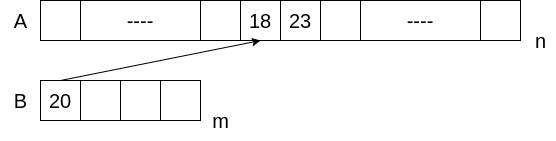
\includegraphics[width=250px]{images/6_Set_intersection/mutual_partitioning.png}
\end{figure}

That's good if at each step we splits up the array $A$ which is not always the case, that's because we try to balance the partitioning: instead of starting from $B[0]$ we start from the element in the middle of $B$ and we search the left part of $B$ in the left part of $A$ and the right part of $B$ in the right part of $A$.
So we exploit the cost of single search to short the cost for next searches.

\subsection{Complexity}
Since $|B| = m$ and on average $|B_1|=|B_2| = \frac{m}{2}$ we have $\#$recursive call of $O(log_2 m)$, the recursive relation is:
$$
    T(n, m) = O(log_2 m) + T\left(n_1, \frac{m}{2}\right) + T\left(n_2, \frac{m}{2}\right)
$$
Let's make some assumptions: in the case of fully unbalanced partitioning, which means that in $A$ the element is found totally on the left or totally on the right, we have a good case because we totally drop half of the array $B$ each time, so the recursive calls will be:
$$
    (n, m) \xrightarrow{} \left(n, \frac{m}{2}\right) \xrightarrow{} \left(n, \frac{m}{4}\right) 
$$
So in this case we have a binary search on a fraction of $B$ and we have $log_2 m$ steps so the complexity in that case is $O(log_2 n \cdot log_2 m)$.

The worst case is when we have fully balanced splitting:
$$
    T(n,m) = O(log_2 m) + T(\frac{n}{2}, \frac{m}{2}) + T(\frac{n}{2}, \frac{m}{2})
$$
whose solution is:
$$
    O\left( m \cdot \left( 1 + log_2 \frac{n}{m} \right) \right)
$$
which can be proved as the optimal solution in the comparison based model for this problem.

\subsubsection{Some observations}
If $n \approx m$ then $\frac{n}{m}$ is a constant value, so:
$$
    O(m \cdot (1+c)) = O(m)
$$
so it is basically merge-based algorithm but in this case merge is better because it uses scan which is better in terms of I/O in respect to random jumping in binary search.

If $m << n$ then the algorithm is:
$$
    O(m \cdot log_2 n)
$$
which basically is binary search.

So this is kinda adaptive to the relation between $m$ and $n$.

\subsection{Proof of lower bound}
In the comparison based model we can use the decision tree technique to calculate the lower bound, and it is given by:
$$
    \Omega(log_2 s(m))
$$
in which $s(m)$ is the $\#$solutions to the problem.

In the case of the intersection problem the number of solution is:
$$
    \binom{n}{m}
$$
so the lower bound is:
$$
    log_2 \binom{n}{m} = m \cdot \left( 1 + log_2 \frac{n}{m} \right)
$$
so that's the proof that mutual partitioning reaches the lower bound for the comparison based model but of course in I/O model it's not since we are jumping around in the memory.

\section{Doubling search}
Doubling search (also known as exponential search or galloping search) states that:
\begin{figure}[H]
    \centering
    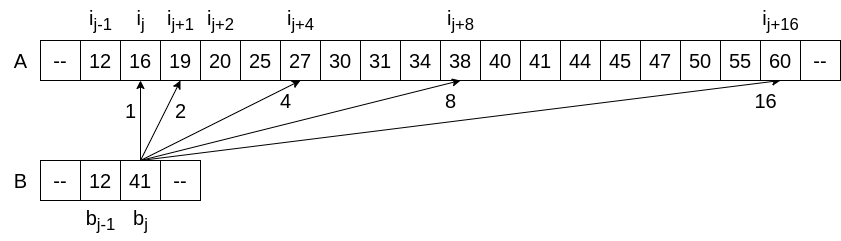
\includegraphics[width=300px]{images/6_Set_intersection/doubling_search.png}
\end{figure}
we go from left to right in order to exploit memory pre-fetch, so we compare 41 with 16, since there is no match and 41 is greater than 16 we go to the next element, we compare 41 to 19, no match here too so we double the distance and go to 27, no match neither here and so we double again the distance going to 38, no match here too, double again the distance and we arrive comparing 41 to 60, no match here too but since 60 is greater than 41 we need to search better, but only in the range between $i_{j+8}$ and $i_{j+16}$.

At each step we double the distance and in the end we will perform a binary search but only on a sub-set, and at each step we reduce the elements we need to check next time!
Moreover we restrict search to an area which has the same size of the area we've discarded, that's very powerful!

\subsection{Complexity}
At each step we do a binary search over $A[i_{j-1} + 2^{k-1}, i_{j-1} + 2^k]$ because:
$$
    A[i_{j-1} + 2^{k-1}] \leq b_j \leq A[i_{j-1} + 2^k]
$$
let's call:
$$
    \Delta_j = min\{ 2^{k-1}, n \} \leq 2^{k}
$$
which is the total size of the elements seen at each step.
Moreover we can state that:
$$
    2^{k-1} \leq i_j - i_{j-1} \leq 2^k
$$
which can be proved by watching at the picture above, so joining the two relations above:
$$
    2^{k-1} \leq i_j - i_{j-1} \implies 2^k \leq 2(i_j - i_{j-1}) \implies \Delta_j < 2(i_j - i_{j-1})
$$

Since sometimes the chunks are overlapped we would like to know how much the overhead can be:
$$
    \sum_{j=1}^m \Delta_j < \sum_{j=1}^m 2(i_j - i_{j-1})
$$
that's a telescopic sum:
$$
    = 2\sum_{j=1}^m i_j - i_{j-1} = 2[(i_1 - i_0) + (i_2 - i_1) + \_ + (i_m - i_{m-1})] = 2[i_m - i_0] = 2i_m \leq 2n
$$
so at the end we have at most $O(n)$ as overlapping part!

Time complexity of each step depends on the jumping part and the binary search one:
$$
    k-1 + log_2 \Delta_j \leq k-1 + log_2 2^{k} = k-1 + k \approx O(k)
$$
in total:
$$
    \sum_{j=1}^m O(k) = \sum_{j=1}^m O(log_2 \Delta_j) = O \left( \sum_{j=1}^m log_2 \Delta_j \right)
$$
we can use the Jensen's inequality:
$$
    \sum_{i=1}^n log_2 x_i \leq n \cdot log_2 \frac{\sum_{i=1}^n x_i}{n}
$$
so we have that:
$$
    O \left( \sum_{j=1}^m log_2 \Delta_j \right) \leq O\left( m \cdot log_2 \frac{\sum_{j=1}^m log_2 \Delta_j}{m} \right) \leq O\left( m \cdot log_2 \frac{2n}{m} \right)
$$
$$    
    = O\left(m \cdot \left(log_2 2 + log_2 \frac{n}{m}\right)\right) = O\left(m \cdot \left(1 + log_2 \frac{n}{m}\right)\right)
$$
So we are reaching the lower bound but again the binary search part is a problem whenever we are taking into account the I/O number!


\section{Two-level approach}
It's an algorithm which promotes scan.
Given the two sequences $A$ and $B$ we pre-process $A$ by splitting the list logically in some blocks of size $L$, then we peek the first item of each partition creating $A'$.
So now we have $|A'| = \frac{n}{L}$ and $A[i \cdot L + 1] = A'[i]$.

Once we have this pre-processing we can execute the actual query $A \cap B$.
First we need to distribute $B$ among the various items of $A'$: we want to know in which of the blocks $A_i$ falls $b_j$. We can of course use a merge approach to do it for each of the elements in $B$.
\begin{figure}[H]
    \centering
    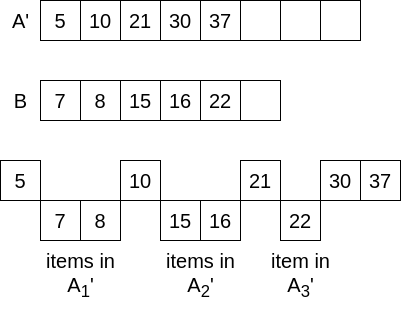
\includegraphics[width=250px]{images/6_Set_intersection/two_level.png}
\end{figure}
As we can see if there are no items between two items from $A'$ we can drop a whole $A$ block.

This algorithm then splits-up array $B$ in single blocks:
$$
    B_i = \{ b \in B : A[i \cdot L + 1] \leq b < A[(i+1) \cdot L] \}
$$
this step costs:
$$
    |A'| + |B| = O\left( \frac{n}{L} + m \right)
$$
and we get $B_i$ and $A_i$.
Of course $B_i$ could even be empty but overall $B = \bigcup_{i} B_i$ so $\sum_{i=1}^{\frac{n}{L}} |B_i| = m$, and $|A_i| = L$.

So now we have restricted the intersection problem to single partitions $A_i$ to $B_i$.
With this strategy we can skip $L$ items with just two comparisons, when using the pre-processed lists!

Now we compute $A_i \cap B_i$ $\forall i=1, 2, \_, \frac{n}{L}$ iff $|B_i| \neq 0$ in a merge-based way to promote scan.
The cost of this step is $O(|A_i| + |B_i|)$ so:
$$
    \sum_{i=1, B_i \neq 0}^{\frac{n}{L}} |A_i| + |B_i| = \sum_{i=1, B_i \neq 0}^\frac{n}{L} |A_i| + \sum_{i=1, B_i \neq 0}^\frac{n}{L} |B_i|
$$
in which the first term can be upper bounded by $m \cdot L$ (because we will scan at most $m$ chunks from $A$, each containing $L$ elements) in the worst case and the second one by $m$ so:
$$
    = O(m \cdot L + m)
$$

NB: another approach could be to shuffle elements using a reversible permutation and then executing the intersection.
That's useful to improve storage because we can store the distance between the elements instead of the real ones.

\subsection{More on 2-level: Interpolation search}
The approach of 2-level memory can be used in a wide variety of solutions, for example we can speed up the search for a key over integers using the interpolation search.
Take the list of elements $X[1, n] = x_1, x_2, \_, x_n$, we calculate $b = \frac{x_n - x_1 + 1}{n}$, it tells us the range of elements that should be inside a single bucket.
Then we build $n$ buckets of size $b$.

For example:
\begin{figure}[H]
    \centering
    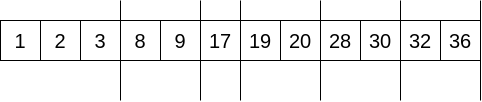
\includegraphics[width=250px]{images/6_Set_intersection/interpolation_search.png}
\end{figure}
Once we've splitted the array in blocks we need to create a structure to store bucket starts and end:
\begin{itemize}
    \item 1, 3: start and end of first block;
    \item 0, 0: no indices since the block is empty;
    \item 4, 5: start and end of third block;
    \item \_
\end{itemize}

\subsubsection{Query}
To search for an item we first need to calculate the index of the block:
$$
    i = \lceil \frac{y - x_1}{b} \rceil + 1
$$
Once we've found the correct block we just need to binary search in it or do a scan.
Supposing of using a binary search the overall cost would be: $O(1 + log_2 b)$, but of course the overall complexity is: $O(1 + log_2 min\{b, n\})$ because it depends on how many items ends up in a bucket, the key space, etc.

This complexity doesn't take into account the distribution of elements, let's define:
$$
    \Delta = \frac{max_i x_i - x_{i-1}}{min_i x_i - x_{i-1}} \geq 1
$$
it's the ratio between the maximum and the minimum gap between two adjacent items.
Then since the maximum is always larger or equal than the average we can state:
$$
    max_i x_i - x_{i-1} \geq \frac{ \sum_{i=2}^n x_i - x_{i-1} }{ n-1 } = \frac{x_n - x_1}{n-1} \geq \frac{x_n - x_1 +1}{n} = b
$$
Then we can estimate the size of a bucket:
$$
    |I_i| \leq n \\
    |I_i| \leq b
$$
but we want something better:
$$
    |I_i| \leq \frac{b}{min_i x_i - x_{i-1}}
$$
because inside a block there can be more of the minimum gap, then each $b$ can be upper bounded by the maximum gap:
$$
    |I_i| \leq \frac{ max_i x_i - x_{i-1} }{ min_i x_i - x_{x-1} } = \Delta
$$
so in each bucket we have at most $\Delta$ items.

So our complexity is at most $O(1 + log_2 \Delta)$ time.

Can be proved that if $X$ is evenly distributed (so elements are spaced by the same amount) and we have $\#$universe $ = U$ and $\#$items $ = n$ then $\Delta = polylog(n)$ with high probability, so:
$$
    O(log_2 \Delta) = O(log_2 log_2^\alpha n) = O(\alpha log_2 log_2 n) = O(log_2 log_2 n)
$$


